%%%%%%%%%%%%%%%%%%%%%%%%%%%%%%%%%%%%%%%%%
% Simple Sectioned Essay Template
% LaTeX Template
%
% This template has been downloaded from:
% http://www.latextemplates.com
%
% Note:
% The \lipsum[#] commands throughout this template generate dummy text
% to fill the template out. These commands should all be removed when 
% writing essay content.
%
%%%%%%%%%%%%%%%%%%%%%%%%%%%%%%%%%%%%%%%%%

%----------------------------------------------------------------------------------------
%	PACKAGES AND OTHER DOCUMENT CONFIGURATIONS
%----------------------------------------------------------------------------------------

\documentclass[12pt]{article} % Default font size is 12pt, it can be changed here

\usepackage{geometry} % Required to change the page size to A4
\usepackage{amsmath}
\usepackage{longtable}
\geometry{a4paper} % Set the page size to be A4 as opposed to the default US Letter

\usepackage{graphicx} % Required for including pictures
\usepackage{caption}
\usepackage{subcaption}

\usepackage{float} % Allows putting an [H] in \begin{figure} to specify the exact location of the figure
\usepackage{wrapfig} % Allows in-line images such as the example fish picture

\usepackage{lipsum} % Used for inserting dummy 'Lorem ipsum' text into the template

\linespread{1.2} % Line spacing

%\setlength\parindent{0pt} % Uncomment to remove all indentation from paragraphs

%\graphicspath{{./Pictures/}} % Specifies the directory where pictures are stored

\begin{document}

%----------------------------------------------------------------------------------------
%	TITLE PAGE
%----------------------------------------------------------------------------------------

\begin{titlepage}

\newcommand{\HRule}{\rule{\linewidth}{0.5mm}} % Defines a new command for the horizontal lines, change thickness here

\center % Center everything on the page

\textsc{\LARGE University of San Diego}\\[1.5cm] % Name of your university/college
\textsc{\Large CS355}\\[0.5cm] % Major heading such as course name
%\textsc{\large Minor Heading}\\[0.5cm] % Minor heading such as course title

\HRule \\[0.4cm]
{ \huge \bfseries Modeling Cloud-Hosting Costs}\\[0.4cm] % Title of your document
\HRule \\[1.5cm]

\begin{minipage}{0.4\textwidth}
\begin{flushleft} \large
\emph{Author:}\\
Nicholas \textsc{Otto} % Your name
\end{flushleft}
\end{minipage}
~
\begin{minipage}{0.4\textwidth}
\begin{flushright} \large
\emph{Professor:} \\
Dr. Simon \textsc{Koo} % Supervisor's Name
\end{flushright}
\end{minipage}\\[4cm]

{\large \today}\\[3cm] % Date, change the \today to a set date if you want to be precise

%\includegraphics{Logo}\\[1cm] % Include a department/university logo - this will require the graphicx package

\vfill % Fill the rest of the page with whitespace
Digital copy and code at https://github.com/ottocode/cs355

\end{titlepage}
\section{Summary}
This report outlines the steps taken to simulate a cloud web hosting company.  
The purpose of the simulation is to determine if there exists a profitable configuration of company parameters, and if so, determine optimal business conditions for the company.  
The simulation was done by carrying out successive simulations designed to isolate the parameters of relative customer provision size, relative customer request size, as well as storage and database reserve requirements.

Ultimately, it was found that the cloud web hosting company can sell over 2.5 times the capacity on hand, with some multiples being as high as 6.15.  
The strategy of adaptively scaling company capacity to the 3 day running average of customer requests was found to be highly effective at keeping pace with demand.  
A minimum of 5\% storage and database reserve is sufficient to satisfy customer demand at least 347 days of the year.
Profitability, as measured by the provisioned level to capacity multiple, increases as customers utilize more of what they provisioned at any given time on average.

In real terms, this means that if the company can compete on price and service by selling provisioning for half of what it costs the company to maintain, then the company will make a profit in every configuration tested here.  In some configurations, the company can sell provisioning for less than 20\% of what is costs to maintain.  This is due to the fact that customers will generally not utilize all of the resources they have provisioned at any given time.

These finding as believed valid for a company with a reasonably stable starting customer base (\(>\) 500).
\newpage

%----------------------------------------------------------------------------------------
%	TABLE OF CONTENTS
%----------------------------------------------------------------------------------------

\tableofcontents % Include a table of contents

\newpage % Begins the essay on a new page instead of on the same page as the table of contents 

%----------------------------------------------------------------------------------------
%	INTRODUCTION
%----------------------------------------------------------------------------------------

\section{Background}
Understanding how a cloud hosting company's system will behave in the face of a dynamic customer population gives not only system administrators, but also financial planners a competitive advantage.
Knowing when to scale resources up or down is an important decision in terms of both finances and operational stability. 
Customers, of course are dynamic, requiring sometimes inconsistent amounts of support.  
This report investigates ways to mitigate the inconsistencies of customer needs by detailing a proactive approach for scaling the technologies behind a cloud hosting platform.
The over-all goal is to minimize the required resources to support an arbitrary customer load, while also minimizing periods when requests exceed capacity.

Cloud hosting, as defined here, consist of three categories: a web server, disk storage, and database operations.
Without much loss of specificity, it is assumed that each category can be broken into finite allocations of resources that are then parceled out to customers as requested.
In other words, this report is not concerned with the finer details of technical specifications, but instead assumes that each category can be "normalized" into some quantity.
\section{Setup}
In describing the technical set-up of the simulation, it is important to first recognize the limitations of this report.
While an understanding of how to most efficiently and profitably operate a start-up cloud hosting company would be very interesting, such a model is beyond our capabilities and scope.
If such a model existed, it is certain that many venture capital firms would be especially interested in the details.
Instead, this report assumes a stable level of customers who have already adopted the cloud hosting service, as well as starting with the capacity to serve those customers.
Without making this assumption, and others noted later, the model devolves into a complete abstraction.

Previously it was mentioned that this report also assumes a "normalization" of resources.  
A "normalization" makes sense for these purposes since it is most interesting to consider customer requests not in real values, but in values relative to the service capacity.
Thinking in this way is intuitive since claiming a set-up that achieves a 4.1 "over-provisioning" is much more meaningful that claiming "316GB over-provisioning."
Thus, to satisfy the initial critical assumption that the modeled cloud hosting company is "stable," it is assumed that the initial conditions are such that the service is likely able to handle the initial round of requests.

The following parameters were varied during the simulation process to determine their effect on the company's profit and service level:
\begin{itemize}
    \item Usage parameter
    \item Provisioning parameter
    \item Storage safety percent
    \item Database safety percent
\end{itemize}

\subsection{Definitions}
The following will be referred to throughout the report:
\begin{center}
    \begin{longtable}{p{4cm} p{10cm}}
        capacity & The level of resources available to the company.\\
        capacity multiplier & Total provisioned by customers / company capacity (averaged over the 3 categories).\\
                 categories & Web Services, Storage Services, and Database services offered by the company.\\
        customer & An entity that has provisioned web, storage, and database services and requests some level of use in each time interval.\\
        over-provisioning & The factor of how much the customers have provisioned over the capacity held by the company.  Over-provisioning \(=\) total-provisioned \(/\) capacity.\\
  storage/database safety & The level of reserve capacity the company attempts to maintain to ensure no storage or database requests cannot be fulfilled.\\
       provision & How much web, storage, and database services a customer has available at any given time (they need not be the same for all three).\\
     utilization & The percentage of capacity used during a time interval.  Utilization \(=\) usage \(/\) capacity.\\
        usage/provisioning parameter & The parameter that defines the skewness towards lower levels of usage or provisioning (see Figure \ref{fig:Provisioning}).

    \end{longtable}
\end{center}
\subsection{Overview}
    The modeled described in this report assumes that each customer will individually request some level of service from each category during a time interval.  The time interval is given as days.  
    The model then sums the aggregate requests of all the customers, and compares the total requests to the total capacity.
    Based on the model parameters, the capacity is then scaled to better service the anticipated requests in the next time interval.
    In any given time interval, up to roughly 30\% of the current customers may leave the service, or become new customers.
    Each simulation lasts 365 days and usage, capacity, and customer statistics are collected throughout.
    The simulation is repeated to vary the initial parameters.

    \subsection{Customer}
    Each customer is given a provisioning and usage parameter that are fixed for an entire simulation, and initialized upon their becoming a customer.
    These parameters specify the probability that the user will request a certain provisioning of the 3 categories and their usage distribution of that provisioning throughout the simulation respectively.
    Based on the author's own experience it was decided to investigate provisioning skewed primarily towards smaller levels.  
    Thus as can be seen from Figure \ref{fig:Provisioning}, the distribution functions for customer provisioning levels are very skewed towards smaller levels of service.
    The provisioning level of a customer is determined by generating a random number from 0 to 1, then applying that random number to the inverse of the distribution function to get the provisioning level.  Note, again, that the provisioning level is in normalized amounts.

    \begin{figure}[h!]
        \centering
        \begin{subfigure}[b]{0.3\textwidth}
            \centering
            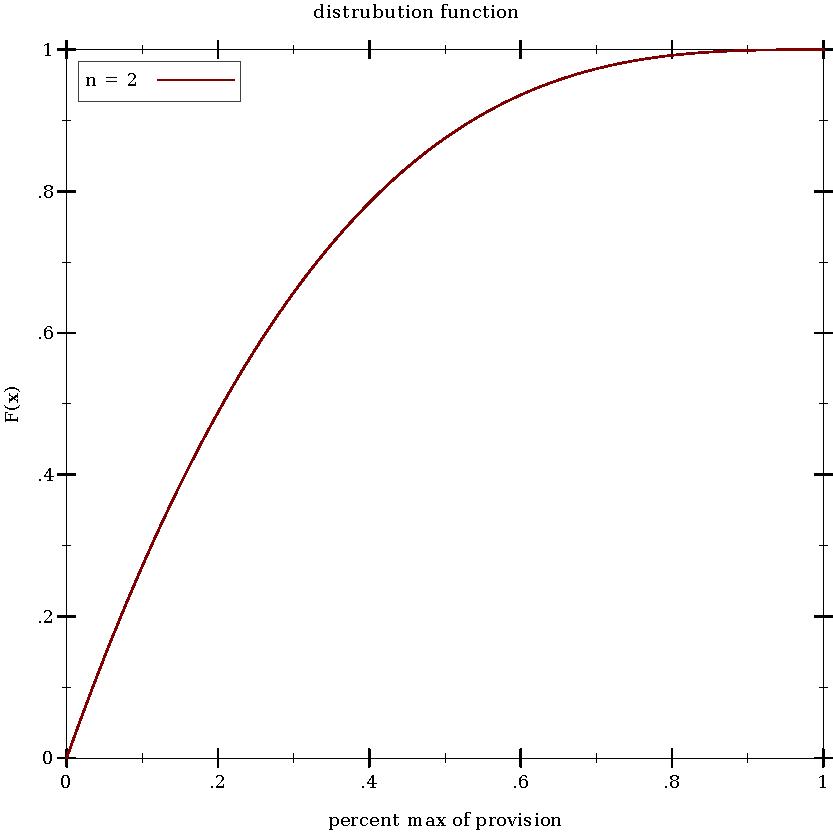
\includegraphics[trim=6cm 0cm 4cm 0cm, scale=0.5]{plots/distribution_out_2.pdf}
            \caption{Provisioning somewhat skewed to smaller amounts, F(0.5) \(\approx\) 0.875.}
            \label{fig:first}
        \end{subfigure}
       \qquad \qquad  \qquad 
        \begin{subfigure}[b]{0.3\textwidth}
            \centering
            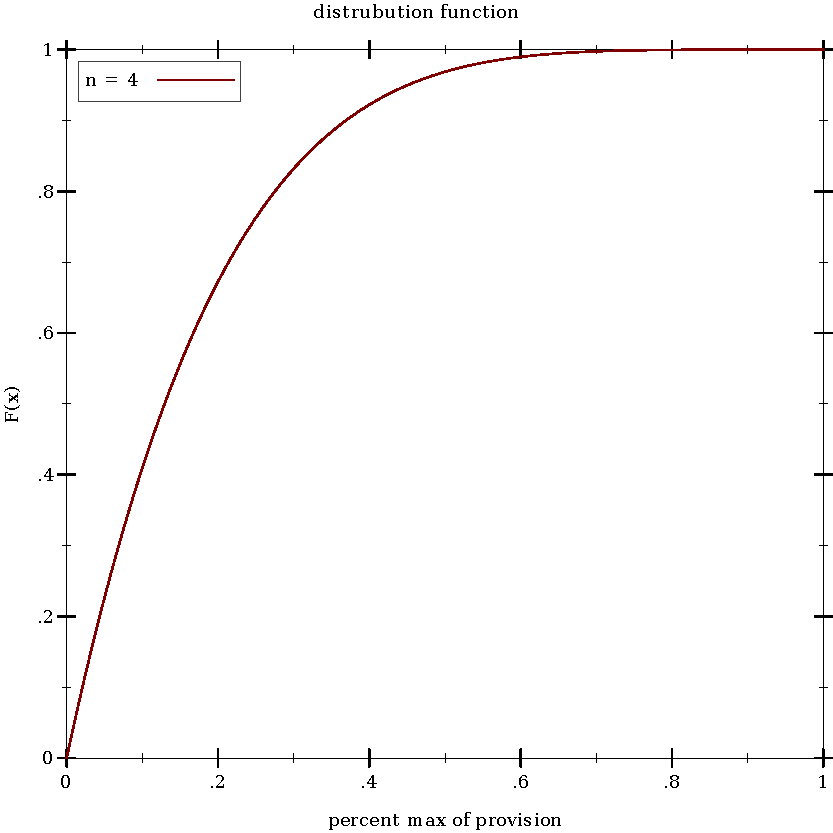
\includegraphics[trim=4cm 0cm 6cm 0cm, scale=0.5]{plots/distribution_out_4.pdf}
            \caption{Provisioning biased towards smaller amounts, F(0.5) \(\approx\) 0.97.}
            \label{fig:second}
        \end{subfigure}

        \vspace{1cm}
        \begin{subfigure}[b]{0.3\textwidth}
            \centering
            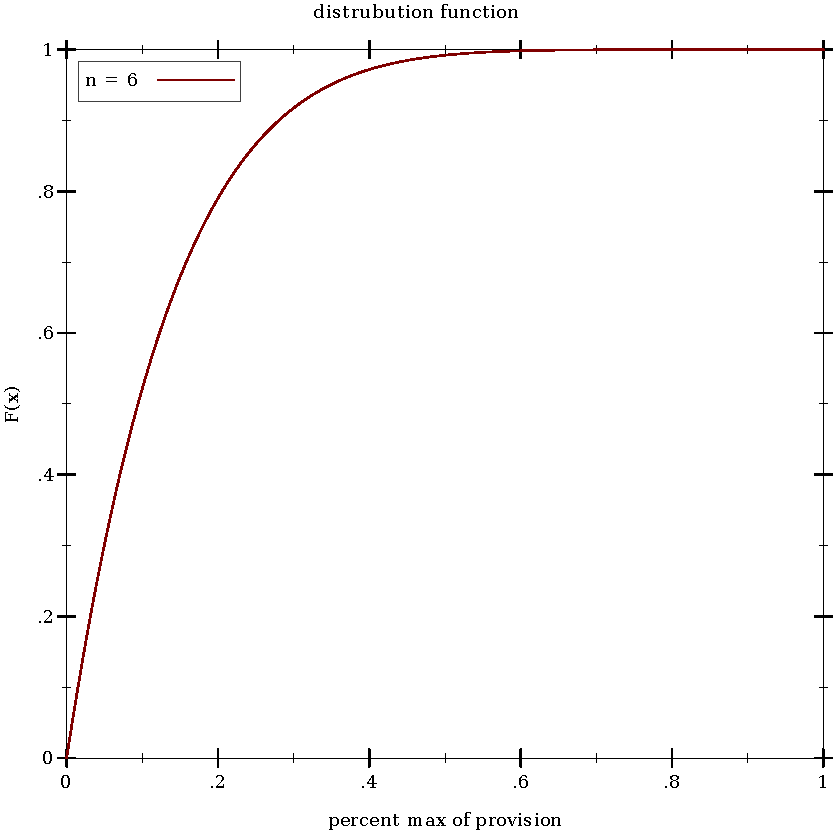
\includegraphics[trim=6cm 0cm 4cm 0cm, scale=0.5]{plots/distribution_out_6.pdf}
            \caption{Provisioning even more skewed to smaller amounts, F(0.5) \(\approx\) 0.992.}
            \label{fig:third}
        \end{subfigure}
       \qquad \qquad  \qquad 
        \begin{subfigure}[b]{0.3\textwidth}
            \centering
            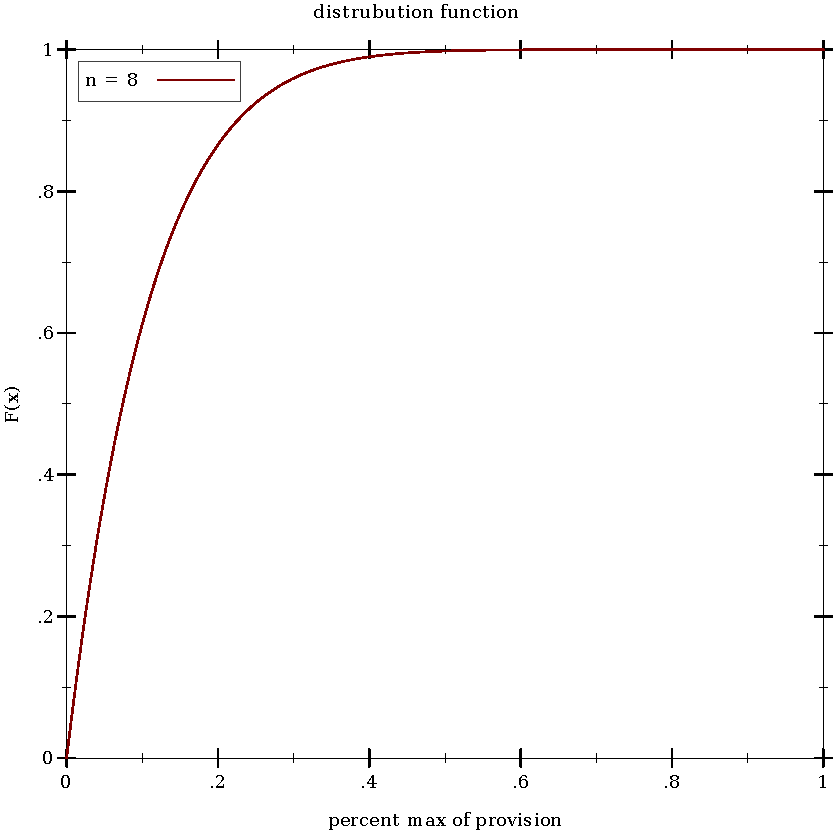
\includegraphics[trim=4cm 0cm 6cm 0cm, scale=0.5]{plots/distribution_out_8.pdf}
            \caption{Provisioning highly skewed to lower amounts, F(0.5) \(\approx\) 0.998.}
            \label{fig:fourth}
        \end{subfigure}

        \caption{Provisioning Distribution Plots for Parameters n = 2, 4, 6, 8.}
        \label{fig:Provisioning}
    \end{figure}

    Determining the usage of each customer in each time interval is done in the exact same fashion as determining the level of provisioning, except that while provisioning is calculated once for each customer for each simulation, usage is calculated for each customer at every time interval.  
    The current usage request is calculated again by the inverse distribution function applied on a random number, which gives the percentage of the customer's provisioned level of service they are requesting during that time interval.

    To simulate the dynamic behavior of customers, at the end of each time interval, the number of customers can change up to 30\% of the current total.  The amount of change is based on the amount of requested services that were unavailable due to lack of capacity during the time interval.  
    The change in customer population is \emph{not} dependent on how much extra capacity is available beyond what is requested (since customers of a web hosting company are unaware of such things).
    The change is calculated as follows:

    The percentage difference between capacity and requests is calculated for each category
    \[
P_{\text{diff}} = \sum_{\text{category}}\frac{\text{total capacity} - \text{total requests}}{\text{total capacity}}.\]
Then if \(R\sim N(1,0.2)\) and \(C = \text{number of customers}\), 
    \[
\Delta_{\text{customers}} = \begin{cases}
    C\cdot 0.3 \cdot \text{max(}P_{\text{diff}}\text{, -1})\cdot R, & P_{\text{diff}} < 0,\\
                          C\cdot 0.005 \cdot R, & P_{\text{diff}} > 0\text{ and short in at least one category},\\
                           C\cdot 0.01 \cdot R, &\text{ otherwise.}
\end{cases}
    \]
    Thus it is clear that the consequences for not delivering enough capacity can be quite harsh and difficult to recover from.

    \subsection{Categories}
    The service categories are the web service, storage, and database services.  
    All three operate mostly the same, except that storage and database services are required to attempt to maintain some level of extra "safety net" in capacity level.
    The reasons for having additional reserves for the storage and database are based on the fact that too little capacity for those services is much more likely to crash the service than a overloaded web server.  Since the customer base is dynamic, the categories must also dynamically update their capacities to handle changes in customer loads.  Rather than a direct sort of "chasing" scheme where the capacity is adjusted to be what it should have been the previous time interval, the categories adjust to a sort of 3 day moving average.

    The daily change is exactly what it is for the customers without the sum:
    \[
P_{\text{catDiff}} = \frac{\text{total capacity} - \text{total requests}}{\text{total capacity}}.\]
This percentage is then averaged over the previous 2 days, \(P_{avg}\), and the resulting capacity is calculated as:
\[\text{Capacity}_\text{new} = \begin{cases} \text{Capacity}_\text{old}\cdot (1-(P_{avg}-\text{safety})) & \text{if }P_{avg} < \text{safety}\\
                                             \text{Capacity}_\text{old}\cdot (1-(P_{avg}-0.1)) & \text{otherwise. }\end{cases}\]
Such a configuration has proven to be very effective at following the true trend of customer requests while maximizing usage and minimizing shortages.\\

Finally, each simulation is allowed to run for 365 days to give an approximation of how the company will look a year later.



\section{Results}

The results are presented in two ways.  First, given all of the assumptions we have enumerated thus far, is this cloud hosting service possible (i.e. can we appropriately scale with users)?
Secondly, if it is possible, what parameters have the greatest effect on profitability for the service?
As a base cut-off, if the storage and database services are overloaded more than 30 days in the year, or if the web service is overloaded more than 10\% more than 30 days in a year, it will be assumed that such a configuration is not suitable for running the company.

\subsection{Scalability}
With the given cut-off, the following results appear:

\begin{itemize}
    \item Every parameter combination except for those that include no database or storage safety provision appear.  Thus for scalability,
    \item usage and provision parameters have no effect,
    \item storage and database safety parameters have no effect after the 5\% safety provision level.
\end{itemize}

\subsection{Optimum Configurations}
The best possible configuration is one where, on average, much more is sold in services than stocked in capacity.  Since we have already achieved a certain level of overloading minimization with the base cut-off, the best possible configuration is a provision parameter of 2, usage parameter of 8, and a safety of 5\%.  
This configuration resulted in 8 overloaded web server days, and 1 overloaded storage or database day.  
The average over-selling multiple of capacity for this optimal configuration was around 6.15 times capacity!


The least optimal configurations were storage and database safeties of 25\% and a usage parameter of 2.  The lowest multiple hovers just above 2.76.  Most interestingly, is the fact that the data, when plotted as capacity multiplier vs utilization, assumes and almost grid-like shape as seen in Figure: \ref{fig:result}.

    \begin{figure}[h]
        \centering
        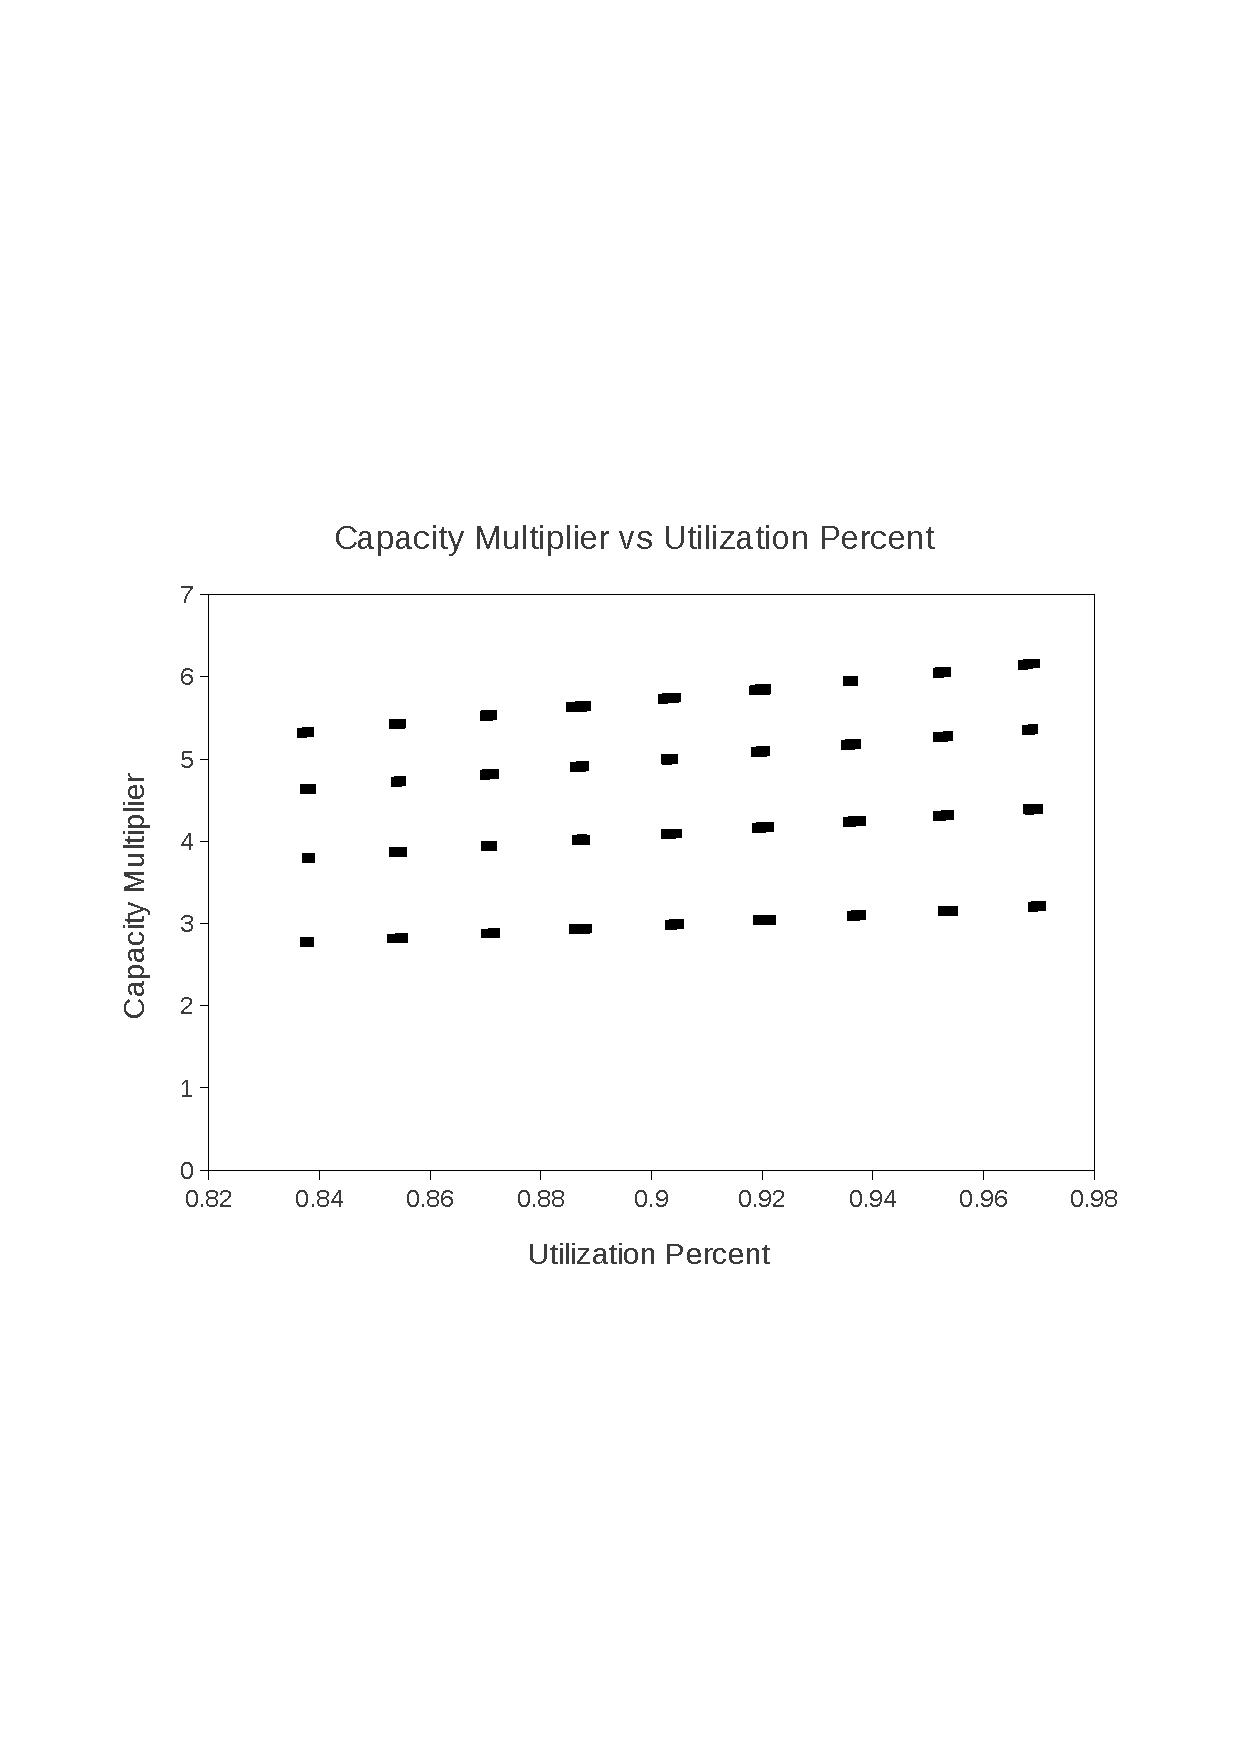
\includegraphics[trim=6cm 8cm 4cm 10cm]{plots/multiplierVSutil.pdf}
        \caption{The data groups together with like usage parameters in this Capacity Multiplier vs Utilization Percent plot.}
        \label{fig:result}
    \end{figure}

    The greatest number of days where either storage or database requests exceeded capacity was 18.


\section{Analysis}
Figure \ref{fig:result} shows that the provisioning parameter has virtually no impact on the capacity multiplier nor utilization percent.  Instead, vertical position (along the capacity multiplier axis) is driven solely by the usage parameter.  Horizontal position in the graph (along the utilization percent axis) is driven by the storage and database safety percentages.  The latter result is intuitive, since if more capacity must be maintained in reserve (higher safety), then the overall utilization of resources should decrease.

While it is not completely intuitive that the provisioning parameter would have no effect on the outcome of the simulation, it is not entirely unrealistic either.  
Indeed, the greater usage parameters indicate that customers are more likely to use less of what they have provisioned, giving more opportunity for a capacity multiplier, regardless of what that original provisioning amount is.

However, the data also shows that to maximize the increase in customers, the total utilization must be minimized (that is the risk of overrunning capacity should be at the absolute minimum).  In fact, the highest capacity multiplier for a customer increase within 10\% of the greatest customer increase is 4.81, a significant decline from the maximum of 6.15.

\section{Conclusions}
Great care must be taken to avoid making too strong a conclusion from these results.  It can be concluded that even with fairly severe "safety" percentages on the storage and database services, the capacity scaling is efficient enough to maintain a healthy capacity multiplier.  The methods presented here, however rely on the assumptions made.  In particular, the assumption that the service is reasonably "stable" must hold.  Without a sizable customer base (about 500), the randomness in the simulation has a much greater effect, and behaves less nicely than the assumptions ultimately presented in this report.  Furthermore, the assumption that users generally consume fractions of what they pay for is key as well.

This report does conclude, however, that a very efficient method of scaling company capacity with consumer variations is not only feasible, but was in fact achieved through the simulations presented here.  
The method of relying on the 3-day moving customer average was very effective at guarding against needless oscillations.  

\end{document}
